%% SECTION HEADER /////////////////////////////////////////////////////////////////////////////////////
\section{High order polynomial interpolation and the \acl{gll} integration scheme}
\label{sec:sem}

%% SECTION CONTENT ////////////////////////////////////////////////////////////////////////////////////

The \ac{sem} is similar to the \ac{fem}.
The similarity of both methods lies in the fact that considered domain is divided into non-overlapping finite elements, and external forces and arbitrary boundary conditions are imposed in the particular nodes.
The main difference between those methods is a selection of the shape function \( N=N(\xi )\), pictured in Figure~\ref{fig:shape}, which is interpolated by a Lagrange polynomial that passes through the element nodes.
The nodes are localised on the endpoint of an interval, \(\xi\in[-1,1]\), and the roots of the first derivative of Legendre polynomial \(\mathcal{P}\) of degree \(p\):
\begin{eqnarray}
	(1-\xi^2)\mathcal{P}'_{p}(\xi)=0.
	\label{eq:nodes}
	\nomtypeD[x]{\( \xi, \eta, \zeta \)}{Local coordinates}{}
	\nomtypeD[w]{\(w\)}{Weighting factor}{}
\end{eqnarray}
The approximation of an integral over the elements is achieved according to the \ac{gll} rule at points coinciding with the element nodes. The integration weights \(w=w(\xi)\) equal
\begin{eqnarray}
	{w(\xi)} = \frac{2}{p(p+1)(\mathcal{P}_{p}(\xi))^2}.
	\label{eq:weight}
\end{eqnarray}

The shape functions and the weights for \ac{2d} or \ac{3d} elements are obtained by the Kronecker product of vectors of individual axes, denoted by \(\otimes\) as follows:
\begin{eqnarray}
	\begin{array}{rcl}
	N(\xi,\eta) & = & N(\xi)\otimes N(\eta),\\
	N(\xi,\eta,\zeta) & = & N(\xi)\otimes N(\eta)\otimes N(\zeta),
	\end{array}
\label{eq:shape_functions}
\nomtypeD[N]{$N$}{Shape function}{}
\end{eqnarray}
\begin{eqnarray}
	\begin{array}{rcl}
	w(\xi,\eta) & = & w(\xi)\otimes w(\eta),\\
	w(\xi,\eta,\zeta) & = & w(\xi)\otimes w(\eta)\otimes w(\zeta).
	\end{array}
	\label{eq:weights}
\end{eqnarray}
\begin{figure}[H]
	\begin{center}
		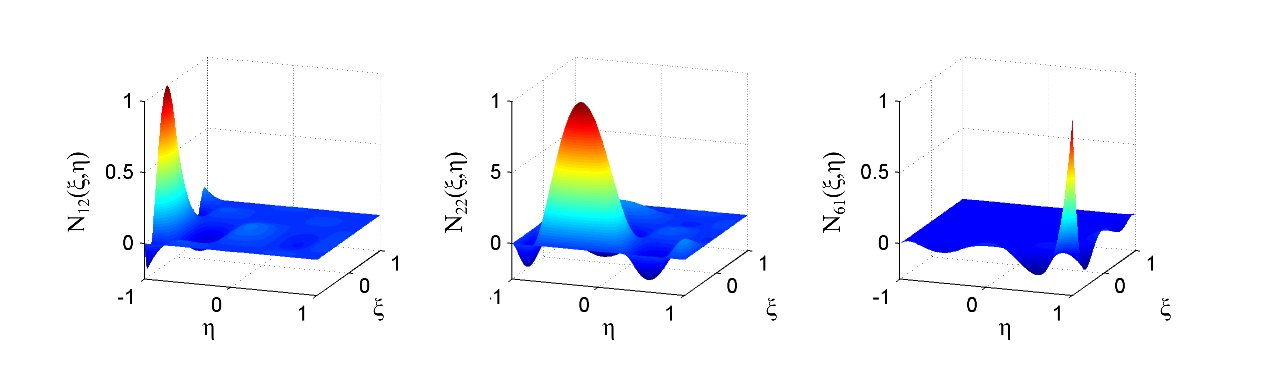
\includegraphics[width=0.95\textwidth]{Chapter_4/shape_function}
	\end{center}
	\caption{Shape functions based on fifth-order polynomial interpolation}
	\label{fig:shape}
\end{figure}

The derivation of the equation of motion is given in \cite{ostachowicz2011guided}, and it is defined as
\begin{eqnarray}
	\label{eq:motion}
	\textbf{M} \ddot{\textbf{d}} + \textbf{D} \dot{\textbf{d}} + \textbf{K} \textbf{d} = \textbf{f}_{ext},
	\nomtypeR[M]{$\textbf{M}$}{Mass matrix}{}{\unit{\kg}}%
	\nomtypeR[D]{$\textbf{D}$}{Damping matrix}{}{\unit[per-mode = symbol]{\newton\second \per \meter}}%
	\nomtypeR[K]{$\textbf{K}$}{Stiffness matrix}{}{\unit[per-mode = symbol]{\newton\per\metre}}%
	\nomtypeR[force_ext]{$\textbf{f}_{ext}$}{External force vector}{}{\unit{\newton}}%
	\nomtypeR[d]{$\textbf{d}$}{Displacements vector}{}{\unit{\meter}}%
\end{eqnarray}
where \textbf{d} is the displacements vector; \textbf{M}, \textbf{D} and \textbf{K} are the structural mass, damping and stiffness matrices, respectively; \textbf{F}$_{ext}$ is the external forces vector; \((\dot{\ })=\frac{\partial}{\partial t}\).
The construction of the structural matrices is similar to the classical approach in \ac{fem}.

The most significant advantage of this method is the fast convergence of the equation of motion.
It is achieved for six nodes per wavelength, while at least fifteen nodes are needed in the case of linear elements in classic \ac{fem}~\cite{wee2017simulating}.
In addition, the mass matrix is diagonal when using the \ac{gll} approach and solid elements or elements based on first-order shear deformation theory.
